% -- tau-transformations
%\newcommand{\smtxtit}[1]{\begin{scriptsize}\ensuremath{\textit{#1}}\end{scriptsize}}
\newcommand{\smtxtit}[1]{\ensuremath{\textit{\scriptsize{#1}}}}
\newcommand{\trans}[1]{\ensuremath{\tau_{#1}}\xspace}
\newcommand{\transtxt}[1]{\trans{\smtxtit{#1}}}
\def\transax{\transtxt{axioms}}
\def\transnorm{\transtxt{norm}}
\def\translt{\transtxt{lt}}
\def\transdlog{\transtxt{datalog}}

\def\LE{\ensuremath{\mathcal{L\!E}}\xspace}
\def\O{\ensuremath{\mathcal{O}}\xspace}
\def\P{\ensuremath{\mathcal{P}}\xspace}
\newcommand{\powset}[1]{\ensuremath{2^{#1}}\xspace}
\def\lprl{\ensuremath{\;:\!-\:}}
\def\cstr{\ensuremath{\;!-\:}}
\def\qury{\ensuremath{\;?-\:}}
\def\dlogrule{\lprl}
\def\dlogcstr{\square\lprl}
\def\dlogand{\wedge}
\def\dlognot{\sim}
\newcommand{\dlogfact}[1]{\ensuremath{{#1}\;.}}

% -- meta-level predicates
\newcommand{\predicate}[1]{\ensuremath{p_{#1}}\xspace}
\newcommand{\predsubtxt}[1]{\mathrm{\sf #1}}
\def\psco{\predicate{\predsubtxt{sco}}}
\def\pmo{\predicate{\predsubtxt{mo}}}
\def\phval{\predicate{\predsubtxt{hval}}}
\def\pitype{\predicate{\predsubtxt{itype}}}
\def\potype{\predicate{\predsubtxt{otype}}}
\def\mlaxioms{\ensuremath{P_{\smtxtit{meta}}}\xspace}

\newcommand{\typeof}{\ensuremath{\textit{typeOf}}\xspace}

\def\bla{\textbf{{\sf bla}}\xspace}

\section{Mapping WSML to Datalog\label{sec:mapping}}
%-- briefly sketch the idea of reasoning via rule based inferencing \\

The semantics of rule-based WSML is defined via a mapping to
Datalog\cite{datalog} with (in)equality and integrity constraints,
as described in \cite{wsml-spec}. To make use of existing rule
engines, the reasoning framework performs various syntactical
transformations to convert an original ontology in WSML syntax
into a semantically equivalent Datalog program. The WSML reasoning
tasks of knowledge base satisfiability and instance retrieval are
then realized by means of Datalog querying via calls to an
underlying Datalog inference engine that is fed with the rules
contained in this program.

% meta-variables.
\def\mvex{\ensuremath{E_x}}
\def\mvey{\ensuremath{E_y}}
\def\mvez{\ensuremath{E_z}}
\def\mve1{\ensuremath{E_1}}
\def\mven{\ensuremath{E_n}}
%\def\mvhd{\ensuremath{H}}
%\def\mvh1{\ensuremath{H_1}}
%\def\mvh2{\ensuremath{H_2}}
%\def\mvhn{\ensuremath{H_n}}
%\def\mvbd{\ensuremath{b}}
%\def\mvb1{\ensuremath{B_1}}
%\def\mvbn{\ensuremath{B_n}}

\subsection{Ontology Transformations}
The transformation of a WSML ontology to Datalog rules forms a
pipeline of single transformation steps which are subsequently
applied, starting from the original ontology.

\paragraph{Axiomatization.} In a first step, the transformation
\transax is applied as a mapping $\O \mapsto \powset{\LE}$ from
the set of all valid rule-based WSML ontologies to the powerset of
all logical expressions that conform to rule-based WSML. In this
transformation step, all conceptual syntax elements, such as
concept and attribute definitions or cardinality and type
constraints, are converted into appropriate axioms specified by
logical expressions. Table \ref{tab:axiomatization} shows the
details of some of the conversions performed by \transax, based on
\cite{wsml-spec}. During the transformation, for each expression
$e$ in the WSML Ontology $O \in \mathcal{O}$ that matches a
pattern on the left-hand side of Table \ref{tab:axiomatization},
the formulae $\transax(e)$ are created and added to the resulting
theory $\transax(O)$.

\begin{table}[]
\centering
\begin{footnotesize}
\begin{tabular}{|l|l|}
  \hline
  \rule{0cm}{3.2mm}{\normalsize \emph{conceptual syntax}} & {\normalsize \emph{logical expression(s)}} \\
  \hline
    $\transax($\wsml{concept} $C_1$ \wsml{subConceptOf} $C_2$ $)$ & $C_1$ \wsml{subConceptOf} $C_2.$ \\
  \hline
      $\transax($\wsml{concept} $C_1$ $A$ \wsml{ofType} $(0,1)$ $T$ $)$ & $C_1$[A \wsml{ofType} $T$]. \\ \ &
      !- ?x \wsml{memberOf} $C_1$ \wsml{and} \\ \ &
      ?x[A \wsml{hasValue} ?y, A \wsml{hasValue} ?z] \\ \ & \wsml{and} ?y != ?z.
      \\
  \hline
      $\transax($\wsml{concept} $C$ & ?x \wsml{memberOf} $C$
      \\ A$_1$ \wsml{inverseOf} A$_2$ \wsml{impliesType} $T$ $)$ & \wsml{and} ?x[A$_1$ \wsml{hasValue} ?v]
      \\ \ & \wsml{implies} ?v \wsml{memberOf} $T$.
      \\ \ & ?x \wsml{memberOf} $C$ \wsml{and}
      \\ \ & ?v \wsml{memberOf} $T$ \wsml{implies}
      \\ \ & ?x[A$_1$ \wsml{hasValue} ?v] \\ \ &
      \wsml{equivalent} ?v[A$_2$ \wsml{hasValue} ?x].
      \\
  \hline
      $\transax($\wsml{relation} $R_1$/$n$
      & $R_1(\vec{x})$ \wsml{implies} $R_2(\vec{x})$. \\
      \wsml{subRelationOf} $R_2$ $)$ &
      where $\vec{x}$ = (x$_1$,...,x$_n$) \\
  \hline
      $\transax($\wsml{instance} $I$ \wsml{memberOf} $C$
      & $I$ \wsml{memberOf} $C$.\\
      A \wsml{hasValue} $V$ $)$ &
      I[A \wsml{hasValue} $V$]. \\
\hline

\end{tabular}
\end{footnotesize}
\caption{Examples for axiomatizing conceptual ontology modeling
elements.} \label{tab:axiomatization}
\end{table}
The meta variables $C,C_i$ range over identifiers of WSML
concepts, $R_i,A_i$ over identifiers of WSML relations and
attributes, $T$ over identifiers of WSML concepts or datatypes.


%To give an example, the WSML fragment
%\begin{lstlisting}[style=wsml]
%concept C subConceptOf D
%    r ofType (0 2) T
%instance a memberOf C
%    r hasValue b,c
%\end{lstlisting}
%is translated by \transax to the following logical expressions.
%\begin{lstlisting}[style=wsml]
%C subConceptOf D. C[r ofType T]. !- ?x memberOf C and ?x[r
%hasValue?y1, r hasValue ?y2] and ?y1 != ?y2. a memberOf C.  a
%hasValue b,c.
%\end{lstlisting}

\paragraph{Normalization.} The transformation \transnorm is
applied as a mapping $\powset{\LE} \mapsto \powset{\LE}$ to
normalize WSML logical expressions. This normalization step
reduces the complexity of WSML logical expressions according to
\cite[Section 8.2]{wsml-spec}, to bring the expressions closer to
the simple syntactic form of literals in Datalog rules. The
reduction includes conversion to negation and disjunctive normal
forms as well as decomposition of complex WSML molecules. Table
\ref{tab:normalization} shows how the various logical expressions
are normalized in detail. The meta variables $E$ range over
logical expressions in rule-based WSML, while $X,Y$ range over
parts of WSML molecules. After \transnorm has been applied, the
resulting WSML logical expressions have the form of logic
programming rules with no deep nesting of logical connectives.

\begin{table}[]\centering
\begin{footnotesize}
\begin{tabular}{|l|l|}
  \hline
  \rule{0cm}{3.2mm}{\normalsize \emph{original expression}} & {\normalsize \emph{normalized expression}} \\
  \hline
    $\transnorm(\{\mve1 , \dots , \mven\})$ & $\{\transnorm(\mve1) , \dots , \transnorm(\mven)\}$ \\
    $\transnorm(\mvex$ \wsml{and} $\mvey.)$ & $\transnorm(\mvex)$ \wsml{and} $\transnorm(\mvey)$ \\
    $\transnorm(\mvex$ \wsml{or} $\mvey.)$ & $\transnorm(\mvex)$ \wsml{or} $\transnorm(\mvey)$ \\
    $\transnorm(\mvex$ \wsml{and} $(\mvey$ \wsml{or} $\mvez).)$ & $\transnorm(\transnorm(\mvex)$ \wsml{and} $\transnorm(\mvey)$ \wsml{or} \\
    & $\phantom{\transnorm(}\transnorm(\mvex)$ \wsml{and} $\transnorm(\mvez).)$ \\
    $\transnorm((\mvex$ \wsml{or} $\mvey)$ \wsml{and} $\mvez).)$ & $\transnorm(\transnorm(\mvex)$ \wsml{and} $\transnorm(\mvez)$ \wsml{or} \\
    & $\phantom{\transnorm(}\transnorm(\mvey)$ \wsml{and} $\transnorm(\mvez).)$ \\
    $\transnorm($ \wsml{naf} $ (\mvex$ \wsml{and} $\mvey).)$ & $$ \wsml{naf} $ \transnorm(\mvex)$ \wsml{or} $$ \wsml{naf} $ \transnorm(\mvey).$ \\
    $\transnorm($ \wsml{naf} $ (\mvex$ \wsml{or} $\mvey).)$ & $$ \wsml{naf} $ \transnorm(\mvex)$ \wsml{and} $$ \wsml{naf} $ \transnorm(\mvey).$ \\
    $\transnorm($ \wsml{naf} $ ($ \wsml{naf} $ \mvex).)$ & $\transnorm(\mvex)$ \\
    $\transnorm(\mvex$ \wsml{implies} $\mvey.)$ & $\transnorm(\mvey)$\wsml{\lprl}$\transnorm(\mvex).$ \\
    $\transnorm(\mvex$ \wsml{impliedBy} $\mvey.)$ & $\transnorm(\mvex)$\wsml{\lprl}$\transnorm(\mvey).$ \\
    $\transnorm(X[Y_1 , \dots , Y_n].)$ & $X[Y_1]$ \wsml{and} $\dots$ \wsml{and} $X[Y_n].$ \\
  \hline
\end{tabular}
\end{footnotesize}
\caption{Normalization of WSML logical expressions.}
\label{tab:normalization}
\end{table}

\paragraph{Lloyd-Topor Transformation.} The transformation
\translt is applied as a mapping $\powset{\LE} \mapsto
\powset{\LE}$ to flatten the complex WSML logical expressions,
producing simple rules according to the Lloyd-Topor
transformations \cite{lloyd-topor}, as shown in Table
\ref{tab:lloyd-topor}.
\begin{table}[tb]
\centering
\begin{footnotesize}
\begin{tabular}{|l|l|}
  \hline
  \rule{0cm}{3.2mm}{\normalsize \emph{original expression}} & {\normalsize \emph{simplified rule(s)}} \\
  \hline
  $\translt( \{ \mve1 , \dots , \mven \})$ & $\{ \translt(\mve1) , \dots , \translt(\mven) \}$ \\
  $\translt(H_1$ \wsml{and} $\dots$ \wsml{and} $H_n$\wsml{\lprl}$B.)$ & $\translt(H_1$\wsml{\lprl}$B.)$ , \dots , $\translt(H_n$\wsml{\lprl}$B.)$ \\
  $\translt(H_1$\wsml{\lprl}$H_2$\wsml{\lprl}$B.)$ & $\translt(H_1$\wsml{\lprl}$H_2$ \wsml{and} $B.)$ \\
  $\translt(H$\wsml{\lprl} $B_1$ \wsml{or} , $\dots$ , \wsml{or} $B_n.)$ & $\translt(H$\wsml{\lprl}$B_1.)$ , \dots , $\translt(H$\wsml{\lprl}$B_n.)$ \\
  \hline
\end{tabular}
% --old tabel with Lloyd-Topor trasnformations
%\begin{tabular}{|c|c|}
%  \hline
%  % after \\: \hline or \cline{col1-col2} \cline{col3-col4} ...
%  \emph{original expression} & \emph{simplified rule(s)} \\
%  \hline
%  $H_1 \wedge \dots \wedge H_n \leftarrow B$ & $H_1 \leftarrow B , \dots , H_n \leftarrow B$ \\
%  $H_1 \leftarrow H_2 \leftarrow B$ & $H_1 \leftarrow H_2 \wedge B$ \\
%  $H \leftarrow B_1 \vee \dots \vee B_n$ & $H \leftarrow B_1 , \dots , H \leftarrow B_n$ \\
%  \hline
%\end{tabular}
\end{footnotesize}
\caption{Lloyd-Topor transformations.} \label{tab:lloyd-topor}
\end{table}
Again, the meta variables $E,H,B$ range over WSML logical
expressions, while $H$ and $B$ match the form of valid head and
body expressions, respectively, according to \cite{wsml-spec}.

After this step, the resulting WSML expressions have the form of
proper Datalog rules with a single head and conjunctive (possibly
negated) body literals.

\paragraph{Datalog Rule Generation.} In a final step, the
transformation \transdlog is applied as a mapping $\powset{\LE}
\mapsto \P$ from WSML logical expressions to the set of all
Datalog programs, yielding generic Datalog rules that represent
the content of the original WSML ontology. In this generic Datalog
program, all remaining WSML-specific language constructs, such as
\wsml{subConceptOf} or \wsml{ofType}, are replaced by special
meta-level predicates for which the semantics of the respective
language construct is encoded in meta-level axioms as described in
a further subsection.
\begin{table}[] \centering
\begin{footnotesize}
\begin{tabular}{|l|l|}
  \hline
  \rule{0cm}{3.2mm} {\normalsize \emph{WSML}} & {\normalsize \emph{Datalog}} \\
  \hline
  $\transdlog(\{\mve1, \dots , \mven\})$ & $\{\transdlog(\mve1), \dots , \transdlog(\mven)\}$ \\
  $\transdlog($ \wsml{\cstr} $B.)$ & $\dlogcstr \transdlog(B)$ \\
  $\transdlog(H.)$ & \dlogfact{\transdlog(H)} \\
  $\transdlog(H$ \wsml{\lprl} $B.)$ & $\transdlog(H) \dlogrule \transdlog(B)$ \\
  $\transdlog(\mvex$ \wsml{and} $\mvey.)$ & $\transdlog(\mvex) \dlogand \transdlog(\mvey)$ \\
  $\transdlog(C_x$ \wsml{subConceptOf} $C_y.)$ & $\psco(C_x,C_y)$ \\
  $\transdlog(I$ \wsml{memberOf} $C.)$ & $\pmo(I,C)$ \\
  $\transdlog(I[a$ \wsml{hasValue} $V].)$ & $\phval(I,a,V)$ \\
  $\transdlog(C[a$ \wsml{impliesType} $T].)$ & $\pitype(C,a,T)$ \\
  $\transdlog(C[a$ \wsml{ofType} $T].)$ & $\potype(C,a,T)$ \\
  $\transdlog($\wsml{r}$(X_1, \dots , X_n).)$ & $r(X_1, \dots , X_n)$ \\
  $\transdlog(X$ \wsml{=} $Y.)$ & $X = Y$ \\
  $\transdlog(X$ \wsml{!=} $Y.)$ & $X \neq Y$ \\
  \hline
\end{tabular}
\end{footnotesize}
\caption{Transformation from logical expressions in rule-based
WSML to Datalog including meta-level predicates.}
\label{tab:LE2datalog}
\end{table}
Table \ref{tab:LE2datalog} shows the mapping from WSML logical
expressions to Datalog including the meta-level predicates \psco,
\pmo, \phval, \pitype and \potype that represent their respective
WSML language constructs as can be seen from the mapping. The meta
variables $E,H,B$ range over WSML logical expressions with a
general, head or body form, while $C,I,a$ denote WSML concepts,
instances and attributes. Variables $T$ can either assume a
concept or a datatype and $V$ stands for either an instance or a
data value, accordingly.

The resulting Datalog rules are of the form $$H \lprl B_1 , \dots
B_n$$ where $H$ and $B_i$ are literals for the head and the body
of the rule, respectively. Body literals can be negated in the
sense of negation-as-failure, which is denoted by $\dlognot B_i$.
As ususal, rules with an empty body represent facts, and rules
with an empty head represent constraints. The latter is denoted by
the head being the empty clause $\square$.

Ultimately, we define the basic\footnote{Later on, the
transformation pipeline is further extended to support datatypes
and debugging features.} transformation $\tau$ for converting a
rule-based WSML ontology into a Datalog program based on the the
single transformation steps introduced before by $ \tau =
\transdlog \circ \translt \circ \transnorm \circ \transax$.

%\begin{displaymath}
%    \tau = \transdlog \circ \translt \circ \transnorm \circ \transax
%\end{displaymath}
As a mapping $\tau: \O \rightarrow \P$, this concatenation of the
single steps is applied to a WSML ontology $O \in \O$ to yield a
semantically equivalent Datalog program $\tau (O) = P \in \P$ when
interpreted with respect to the meta-level axioms discussed next.

\subsection{WSML Semantics through Meta-Level Axioms}
\label{sec:meta}
%-- describe how a fixed set of rules implements (part of) the WSML semantics during reasoning \\
%-- -- each WSMl entity is mapped to a datalog constant \\
%-- -- special meta-level predicates stand for specific WSMl constructs with a certain semantics; they are applied to datalog constants (give example in picture) \\
%-- -- a direct mapping would not facilitate metamodelling as a feature of WSML \\
%-- -- meta-level axioms assure that the proper semantics of the wSMl constructs is maintained \\
%-- -- the meta-level axioms form rules for the meta-level predicates (, which appear in these rules) \\
%-- -- explain the intuition behind the various meta-level axioms \\

The mapping from WSML to datalog in the reasoning framework works
such that each WSML-identifiable entity, i.e.\ concept, instance,
attribute etc., is mapped to an instance (or logical constant) in
datalog, as depicted in Figure \ref{fig:meta}. There, the concepts
$C_1, C_2, C_3$ as well as the instances $I_1, I_2$ and the
attribute $a$ are mapped to constants such as $I_{C_1}$, $I_{I_1}$
or $I_a$ in datalog, representing the original WSML entities on
the instance level.

Accordingly, the various special-purpose relations that hold
between WSML entities, such as \wsml{subConceptOf},
\wsml{memberOf} or \wsml{hasValue}, are mapped to datalog
predicates that form a meta-level vocabulary for the WSML language
constructs. These are the meta-level predicates that appear in
Table \ref{tab:LE2datalog}, and which are applied to the datalog
constants that represent the WSML entities. The facts listed in
Figure \ref{fig:meta} illustrate the use of the meta-level
predicates. For example, the predicate \psco takes two datalog
constants as arguments that represent WSML concepts, to state that
the concept represented by the first argument is a subconcept of
the one represented by the second argument; on the other hand, the
predicate \pmo takes a datalog constant that represents a WSML
instance and one that represents a WSML concept, to state that the
instance is in the extension of this concept.

In contrast to a direct mapping from WSML to datalog with
concepts, attributes and instances mapping to unary predicates,
binary predicates and constants, respectively, this indirect
mapping allows for the WSML metamodelling facilities.
Metamodelling allows an entity to be a concept and an instance at
the same time. By representing a WSML entity as a datalog
constant, it could, for example, fill both the first as well as
the second argument of e.g.\ the predicate \pmo, in which case it
is interpreted as both an instance and a concept at the same time.

\begin{figure}[tb]
        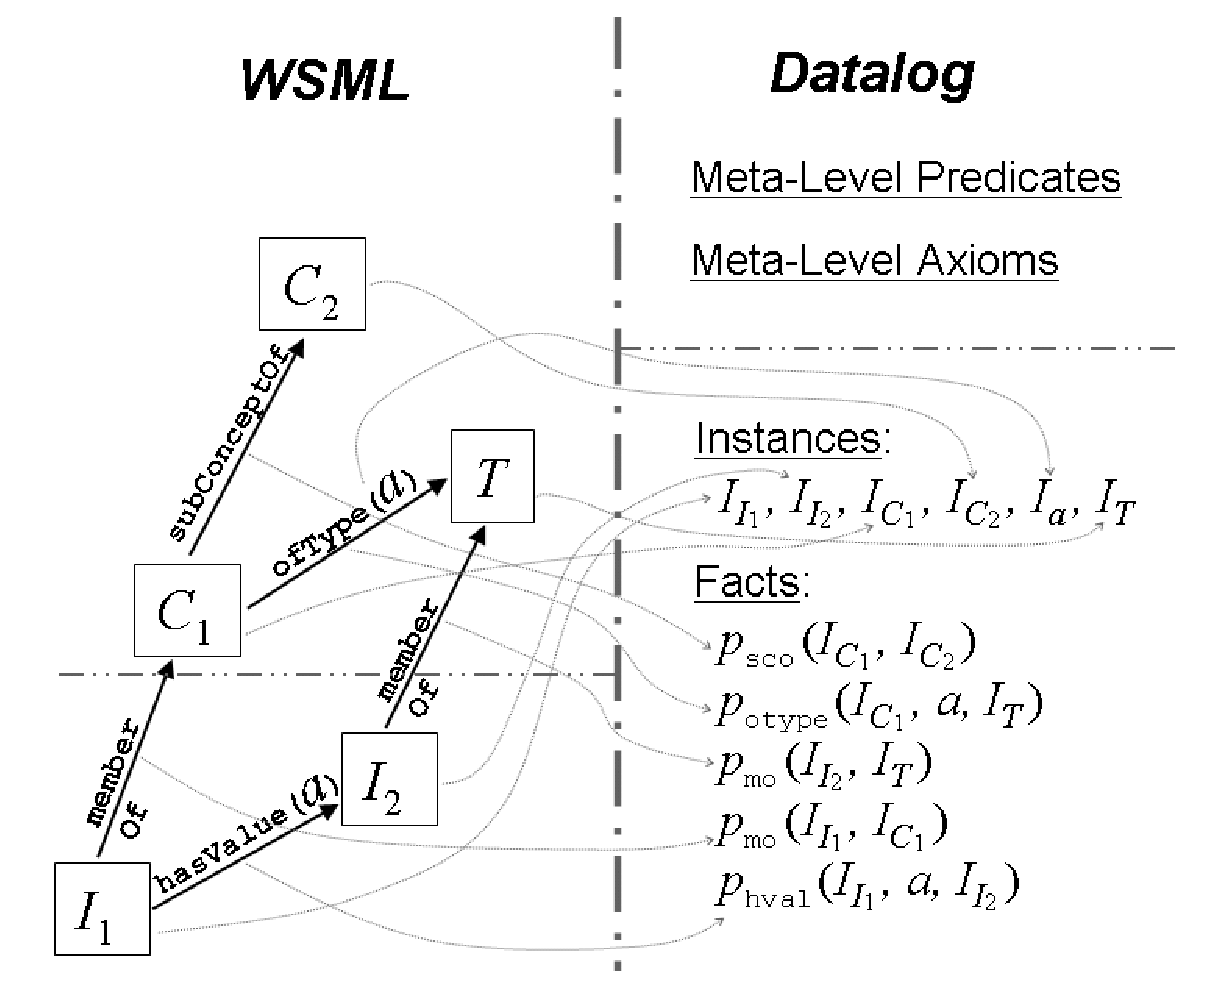
\includegraphics[width=8cm]{figures/meta}
        \centering
    \caption{Usage of meta-level predicates. \label{fig:meta}}
\end{figure}

% -- old table for meta-level predicates + meta-level axioms
%\def\filler{\phantom{l}}
%\begin{table}[tb]\label{tab:meta-level}\centering
%\begin{tabular}{|l|l|}
%  \hline
%  \multicolumn{2}{|l|}{\emph{Meta-Level Predicates}} \\
%  \filler \begin{small}Predicate\end{small} & \begin{small}WSML construct\end{small} \\
%  \hline
%  \filler $\psco(C_{sub},C_{sup})$ \qquad\qquad & $C_{sub}$ \wsml{subConceptOf} $C_{sup}$ \\
%  \filler $\pmo(I,C)$ & $I$ \wsml{memberOf} $C$ \\
%  \filler $\phval(I,a,V)$ & $I[a$ \wsml{hasValue} $V]$ \\
%  \filler $\pitype(C,a,T)$ & $C[a$ \wsml{impliesType} $T]$ \\
%  \filler $\potype(C,a,T)$ & $C[a$ \wsml{ofType} $T]$ \\
%  \hline\hline
%  \multicolumn{2}{|l|}{\emph{Meta-Level Axioms}} \\
%  \hline
%  \multicolumn{2}{|l|}{\filler $\psco(C_1,C_3) \leftarrow \psco(C_1,C_2) \wedge \psco(C_2,C_3)$} \\
%  \multicolumn{2}{|l|}{\filler $\pmo(I,C_2) \leftarrow \pmo(I,C_1) \wedge \psco(C_1,C_2)$} \\
%%  \multicolumn{2}{|l|}{\filler $\pmo(V,C_2) \leftarrow \pitype(C_1,a,C_2) \wedge \pmo(I,C_1) \wedge \phval(I,a,V)$} \\
%  \multicolumn{2}{|l|}{\filler $\pmo(V,C_2) \leftarrow \pitype(C_1,a,C_2) \wedge \pmo(I,C_1)$} \\
%  \multicolumn{2}{|l|}{\filler \phantom{$\pmo(V,C_2) \leftarrow$} \qquad $\wedge \phval(I,a,V)$} \\
%%  \multicolumn{2}{|l|}{\filler $ \leftarrow \potype(C_1,a,C_2) \wedge \pmo(I,C_1) \wedge \phval(I,a,V) \wedge \neg \pmo(V,C_2)$} \\
%  \multicolumn{2}{|l|}{\filler $ \leftarrow \potype(C_1,a,C_2) \wedge \pmo(I,C_1)$} \\
%  \multicolumn{2}{|l|}{\filler $ \phantom{\leftarrow} \qquad \wedge \phval(I,a,V) \wedge \neg \pmo(V,C_2)$} \\
% \hline
%\end{tabular}
%\caption{Meta-level axioms and predicates for WSML semantics in
%datalog.}
%\end{table}
\begin{table}[tb]\label{tab:meta-level}\centering
\begin{small}
\begin{tabular}{|ll|}
  \hline
  \multicolumn{2}{|l|}{\rule{0cm}{3.2mm}{\normalsize \emph{Meta-Level Axioms}}} \\
  \hline
  (1) & $\psco(C_1,C_3) \dlogrule \psco(C_1,C_2) \dlogand \psco(C_2,C_3)$ \\
  (2) & $\pmo(I,C_2) \dlogrule \pmo(I,C_1) \dlogand \psco(C_1,C_2)$ \\
  (3) & $\pmo(V,C_2) \dlogrule \pitype(C_1,a,C_2) \dlogand \pmo(I,C_1)$ \\
  & \phantom{$\pmo(V,C_2) \dlogrule$} $\dlogand \phval(I,a,V)$ \\
  (4) & $\dlogcstr \potype(C_1,a,C_2) \dlogand \pmo(I,C_1)$ \\
  & \phantom{$\dlogcstr$} $\dlogand \phval(I,a,V) \dlogand \dlognot \pmo(V,C_2)$ \\
 \hline
\end{tabular}
\end{small} \caption{Realising WSML semantics in
Datalog.}
\end{table}

A fixed set \mlaxioms of datalog rules forms the meta-level axioms
which assure that the proper semantics of the WSML language is
maintained. In these axioms, the meta-level predicates are
interrelated according to the semantics of the different language
constructs. Table \ref{tab:meta-level} shows the rules that make
up the meta-level axioms in \mlaxioms. Axiom (1) realizes
transitivity for the WSML \wsml{subConceptOf} construct, while
axiom (2) ensures that an instance of a subconcept is also an
instance of its superconcepts. Axiom (3) realizes the semantics
for the \wsml{implisType} construct for attribute ranges: any
attribute value is concluded to be in the extension of the range
type declared for the attribute. Finally, axiom (4) realizes the
semantics of the \wsml{ofType} construct by a constraint that is
violated whenever an attribute value cannot be concluded to be in
the extension of the declared range type.

\subsection{WSML Reasoning by Datalog Queries}
%-- describe how to realise WSML satisfiability and entailment through datalog querying \\
%-- -- characterize the KB (datalog program) on which reasoning is performed with the different facts and rules  \\
%-- -- show how the WSML reasoning tasks are mapped to datalog queries (KB sat., entailment and conjunctive query answering) \\

To perform reasoning over the original WSML ontology $O$ with an
underlying datalog inference engine, a datalog program
\begin{displaymath}
    P_O = \mlaxioms \cup \tau(O)
\end{displaymath}
is built up that consists of the meta-level axioms together with
the transformed ontology. The different WSML reasoning tasks are
then realized by performing Datalog queries on $P_O$. Posing a
query $Q(\vec{x})$ to a Datalog program $P \in \P$ is denoted by
$$(P,\qury Q(\vec{x}))$$ and yields a set of tuples that instantiate
the vector $\vec{x}$ of variables in the query.

\paragraph{Ontology Consistency} -- The task of checking a WMSL
ontology for consistency is done by querying for the empty clause,
as expressed by the following equivalence.
\begin{displaymath}
    O \; \textrm{\footnotesize{is satisfiable}} \; \Leftrightarrow \; (P_O , \qury \square) =
    \emptyset
\end{displaymath}
If the resulting set is empty then the empty clause could not be
derived from the program and the original ontology is satisfiable,
otherwise it is not.

\paragraph{Entailment} -- The reasoning task of entailment of
ground facts by a WSML ontology can be done by using queries that
contain no variables, as expressed in the following equivalence.
\begin{displaymath}
    O \models \phi \; \Leftrightarrow \; (P_O, \qury
    \tau'(\phi')) \not= \emptyset
\end{displaymath}
From the WSML ground fact $\phi \in \LE$ we derive a non-ground
formula $\phi' \in \LE$ by replacing the left-most occurrence of a
constant by the variable $x$. $\phi'$ is then transformed to
Datalog with a transformation $\tau' = \transdlog \circ \translt
\circ \transnorm$, similar to the one that is applied to the
ontology, and is evaluated together with the Datalog program
$P_O$. If the resulting set is non-empty then $\phi$ is entailed
by the original ontology, otherwise it is not.

\paragraph{Retrieval} -- Similarly, instance retrieval can be
performed by posing queries that contain variables to the Datalog
program $P_O$, as expressed in the following equivalence.
\begin{displaymath}
   % \{\vec{x} : O \models Q(\vec{x})\} \; \Leftrightarrow \; (P_O, \qury \tau(Q(\vec{x})))
   retrieve_O(Q) \; = \; (P_O, \qury \tau'(Q(\vec{x})))
\end{displaymath}
The query $Q(\vec{x})$, formulated as a WSML logical expression
with free variables $\vec{x}$, is transformed to Datalog and
evaluated together with the program $P_O$. The resulting set
contains all tuples $\vec{x}$ for which an instantiation of the
query expression is entailed by the original ontology.
To give an example, the query $Q($\syn{?x}$)$ = \\
\phantom{mmmmm} \syn{?x} \synkw{memberOf} \syn{BroadbandBundle}\\
posed to the ontology in Listing \ref{lst:wsml-ontology-example}
yields the set $\{ (\textit{MyBundle}) \}$ that contains one unary
tuple with the instance \textit{MyBundle}, which can be inferred
to be a broadband bundle due to its high network bandwidth.

%\begin{small}
%\begin{tabular}{|l|l|}
%  \hline
%  $O$ is satisfiable & $(P_O, \qury \dlognot \square) \rightarrow \top$ \\
%  $O \models \phi(\vec{C})$ & $(P_O, \qury \phi(\vec{C})) \rightarrow \top$ \\
%  $\{\vec{X} : O \models Q(\vec{X})\}$ & $\{\vec{X} : (P_O, \qury Q(\vec{X})) \rightarrow \top\}$ \\
% \hline
%\end{tabular}
%\end{small}
%
%( $\phi_g$ : ground fact ; $\vec{X}$ : variable binding )

\subsection{Realising Datatype Reasoning}
-- describe how reasoning with datatypes is realised As a result
of the transformations described previously, a generic Datalog
program is created. This generic program cannot be executed,
however, on a particular Datalog implementation without any
changes. Although most of the Datalog rules are understood by any
Datalog implementations, realizing datatype reasoning has some
intricate challenges.

To demonstrate the problems with datatype reasoning, consider the
ontology snippet shown in Figure~\ref{fig:datatype_example}.

\begin{figure}[hbt]
\centering
\begin{lstlisting}[style=wsml, frame=none]
concept Humanoid
  heightInFeet ofType _decimal

//Humanoids that are bigger than 7 feet are big
axiom bigHumanoidDefinition definedBy BigHumanoid(?x) :- ?x
memberOf Humanoid and ?x[heightInFeet hasValue ?v] and ?v > 7.0.

instance arwen memberOf Humanoid
  heightInFeet hasValue 5.5

instance aragorn memberOf Humanoid
  heightInFeet hasValue "big"
\end{lstlisting}
 \caption{Datatype example. \label{fig:datatype_example}}
\end{figure}

It is easy to see that the definition of \syn{aragorn} is not
correct, because the constant "big" is not a decimal number. I.e.,
the ontology is not satisfiable. On the other hand, the definition
of \syn{arwen} is correct, because $5.5$ is a decimal number.

The constraint that should check the datatype constraint on
\syn{heightInFeet} is the following, according Axiom (4) in
Table~\ref{tab:meta-level}:
\begin{displaymath}
    \leftarrow \potype(Humanoid,heightInFeet,_decimal) \wedge \\
    \phantom{\leftarrow} \pmo(I,Humanoid) \\
  \phantom{\leftarrow} \wedge \phval(I,heightInFeet,V) \\
  \phantom{\leftarrow} \wedge \neg \pmo(V,_decimal)
\end{displaymath}

The problem is that during the transformation steps no $\neg
\pmo(V,_decimal)$ statement is generated, because datatype
constants such as $5.5$ or "big" are built-in constructs, and no
explicit axioms state their type. As a result, the constraint will
be always violated whenever the \syn{heightInFeet} attribute has a
value; independently from the fact whether the value is correct
(as in the case of \syn{arwen}) or incorrect (as in the case of
\syn{aragorn}).

To solve this problem, \pmo facts for all datatype constants that
appear in the ontology should be generated. I.e., for each
constant in the ontology axioms of the following form should
appear:
\begin{displaymath}
    \pmo(V,D) \wsml{\lprl} \typeof(V, D_T)
\end{displaymath} where $D$ denotes the WSML datatype, $D_T$ denotes a datatype supported by the underlying Datalog implementation, which is compatible with the WSML datatype, and \typeof denotes a built-in predicate implemented by the Datalog tool, which checks whether a constant value belongs to the specified datatype.

Including such axioms into the tool-specific Datalog program
yields the correct result that the definition of \syn{aragorn}
violates the \synkw{ofType} constraint, while the definition of
\syn{arwen} does not.

WSML also supports some built-in predicates on datatypes, such as
numeric comparison\footnote{A full list of WSML datatypes can be
found in the WSML specification \cite{wsml-spec}.}. E.g., the
definition of \syn{BigHumanoid} uses a shortcut of the WSML
\synkw{numericGreaterThan} predicate. Clearly, these special WSML
predicates have to be translated to the corresponding built-in
predicates supported by the built-in Datalog reasoner.

To summarize the discussion, the underlying Datalog implementation
must fulfill the following requirements to support WSML datatype
reasoning:
\begin{itemize}
    \item It should provide built-in datatypes that correspond to WSML built-in datatypes.
    \item It should provide a predicate (or predicates) for checking the datatype of a constant.
    \item It should provide built-in predicates that correspond to WSML built-in predicates.
\end{itemize}

The main Datalog engine we used during our work was the KAON2
inference engine\footnote{KAON2 is available for download from
\url{http://kaon2.semanticweb.org}} \cite{hustadt04reducing}.
KAON2 provides a very flexible type system that allows for
user-defined datatypes, together with user-defined predicates on
these datatypes, including type checking predicates. Therefore,
KAON2 meets the identified requirements easily. As a matter of
fact, KAON2 already provided most of the required datatypes and
predicates out of the box. Of course, any other Datalog
implementation, can be used that fulfills the requirements (such
as MINS (TODO: insert reference here)).

